\chapter{Luyện tập: Suất điện động cảm ứng}
\begin{enumerate}
	\item
	{
		Cuộn dây có $N=100$ vòng, mỗi vòng có diện tích $S=\SI{300}{\centi \meter \squared}$, đặt trong từ trường đều có cảm ừng từ $B=\SI{0.2}{\tesla}$ sao cho trục của cuộn dây song song với các đường sức từ. Quay đều cuộn dây để sau $\Delta t= \SI{0.5}{\second}$ trục của nó vuông góc với các đường sức từ thì độ lớn suất điện động cảm ứng trung bình trong cuộn dây là
		\begin{mcq}(4)
			\item{$\SI{0.6}{\volt}$.}
			\item{$\SI{1.2}{\volt}$.}
			\item{$\SI{3.6}{\volt}$.}
			\item{$\SI{4.8}{\volt}$.}
		\end{mcq}
	}
	\item
	{
		Một khung dây có $100$ vòng được đặt trong từ trường đều sao cho các đường sức từ vuông góc với mặt phẳng của khung dây. Diện tích của mỗi vòng dây là $\SI{2}{\deci \meter \squared}$, cảm ứng từ giảm đều từ $\SI{0.5}{\tesla}$ đến $\SI{0.2}{\tesla}$ trong thời gian $\SI{0.1}{\second}$. Suất điện động cảm ứng trong khung dây là
		\begin{mcq}(4)
		\item{$\SI{6}{\volt}$.}
		\item{$\SI{60}{\volt}$.}
		\item{$\SI{3}{\volt}$.}
		\item{$\SI{30}{\volt}$.}
		\end{mcq}
	}
	\item
	{
		Một khung dây hình vuông có cạnh $\SI{5}{\centi \meter}$, đặt trong từ trường đều $\SI{0.08}{\tesla}$, mặt phẳng khung dây vuông góc với các đường sức từ. Trong thời gian $\SI{0.2}{\second}$, cảm ứng từ giảm xuống đến $0$. Độ lớn của suất điện động cảm ứng trong khung trong khoảng thời gian đó là
		\begin{mcq}(4)
		\item{$\SI{0.04}{\milli \volt}$.}
		\item{$\SI{0.5}{\milli \volt}$.}
		\item{$\SI{1}{\milli \volt}$.}
		\item{$\SI{8}{\volt}$.}
		\end{mcq}
	}
	\item
	{
		Một khung dây có $1000$ vòng được đặt trong từ trường đều sao cho các đường sức từ vuông góc với mặt ohẳng của khung. Diện tích mặt phẳng giới hạn bởi mỗi vòng là $\SI{2}{\deci \meter \squared}$. Cảm ứng từ của từ trường giảm đều từ $\SI{0.5}{\tesla}$ đến $\SI{0.2}{\tesla}$ trong thời gian $\SI{0.1}{\second}$. Độ lớn suất điện động cảm ứng xuất hiện trong khung là
		\begin{mcq}(4)
		\item{$\SI{60}{\volt}$.}
		\item{$\SI{80}{\volt}$.}
		\item{$\SI{160}{\volt}$.}
		\item{$\SI{50}{\volt}$.}
		\end{mcq}	
	}
	\item
	{
		[Đề chính thức của BGD-ĐT-2018] Một vòng dây kín, phẳng được đặt trong từ trường đều. Trong khoảng thời gian $\SI{0.02}{\second}$, từ thông qua vòng dây giảm đều từ giá trị $\SI{4e-3}{\weber}$ về $0$ thì suất điện động cảm ứng xuất hiện trong vòng dây có độ lớn
		\begin{mcq}(4)
			\item{$\SI{0.2}{\volt}$.}
			\item{$\SI{8}{\volt}$.}
			\item{$\SI{2}{\volt}$.}
			\item{$\SI{0.8}{\volt}$.}
		\end{mcq}
	}
	\item
	{
		Thanh kim loại AB dài $\SI{20}{\centi \meter}$ kéo trượt đều trên hai thanh ray kim loại nằm ngang như hình vẽ.
		\begin{center}
		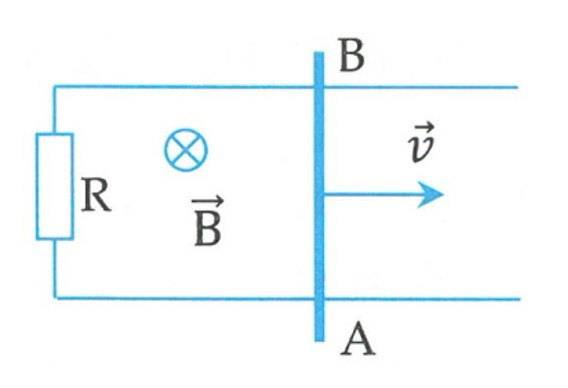
\includegraphics[scale=0.4]{../figs/VN11-PH-30-P-0201-1.jpg}
		\end{center}
		Các dây nối nhau bằng điện trở $R=\SI{3}{\Omega}$. Vận tốc của thanh AB là $\SI{12}{\meter / \second}$. Hệ thống đặt trong từ trường đều có $B=\SI{0.4}{\tesla}$, $\vec{B}$ vuông góc với mạch điện.
		\begin{description}
			\item[a)] Tìm suất điện động cảm ứng trong khung.
		\begin{mcq}(4)
			\item{$\SI{0.48}{\volt}$.}
			\item{$\SI{0.96}{\volt}$.}
			\item{$\SI{0.83}{\volt}$.}
			\item{$\SI{0.69}{\volt}$.}
		\end{mcq}
			\item[b)] Tính cường độ dòng điện cảm ứng và cho biết chiều của dòng điện cảm ứng.
		\begin{mcq}(2)
			\item{$I_\text c=\SI{0.32}{\ampere}$ và chiều từ A đến B.}
			\item{$I_\text c=\SI{0.32}{\ampere}$ và chiều từ B đến A.}
			\item{$I_\text c=\SI{0.23}{\ampere}$ và chiều từ A đến B.}
			\item{$I_\text c=\SI{0.23}{\ampere}$ và chiều từ B đến A.}
		\end{mcq}
		\end{description}
	}
\end{enumerate}
\hides{\textbf{Đáp án}
\begin{center}
	\begin{tabular}{|m{2.8em}|m{2.8em}|m{2.8em}|m{2.8em}|m{2.8em}|m{2.8em}|m{2.8em}|m{2.8em}|m{2.8em}|m{2.8em}|}
		\hline
		1. B & 2. A & 3. C & 4. A & 5. A & 6a. B & 6b. A &&&\\
		\hline
	\end{tabular}
\end{center}}